\chapter{Introduction}
\label{chap:intro}
Ancient papyri are frequently torn into several fragments, and the task of papyrologists is to assemble
and decipher these fragments. Once successfully reconstructed, ancient papyrus offers the opportunity
to gather crucial information about past times. However, reassembling by hand is time-consuming
because fragments differ in color, structure, and shape. Since the phrase puzzling is used, it implies that those fragments are perfectly designed puzzle pieces. Usually, it is the opposite. That means that non-professionals can not tell if two images belong together at all. An example is shown in Figure \ref{fig:papyri_sample}. It can be observed from the Figure that the fibers, the color, and the structure of the two fragments do not fit perfectly into each other. Nevertheless, they belong to the same papyrus. It is hard to tell whether fragments belong together or not because they age differently. Environmental local factors such as exposure to sunlight determine the altering process differently. For example, the medium color of two fragments is inconsistent if one fragment was buried and the second fragment was not. That implies that color is not a good feature for matching fragments.\\
Finding meaningful features (semi) automatically on historical documents and reassembling them has become a popular challenge in the computer vision community. The researchers apply machine learning algorithms to the data and train a model. Those models can then find potential matching candidates for a specific fragment.
\begin{figure}[t]
	\label{fig:papyri_sample}
	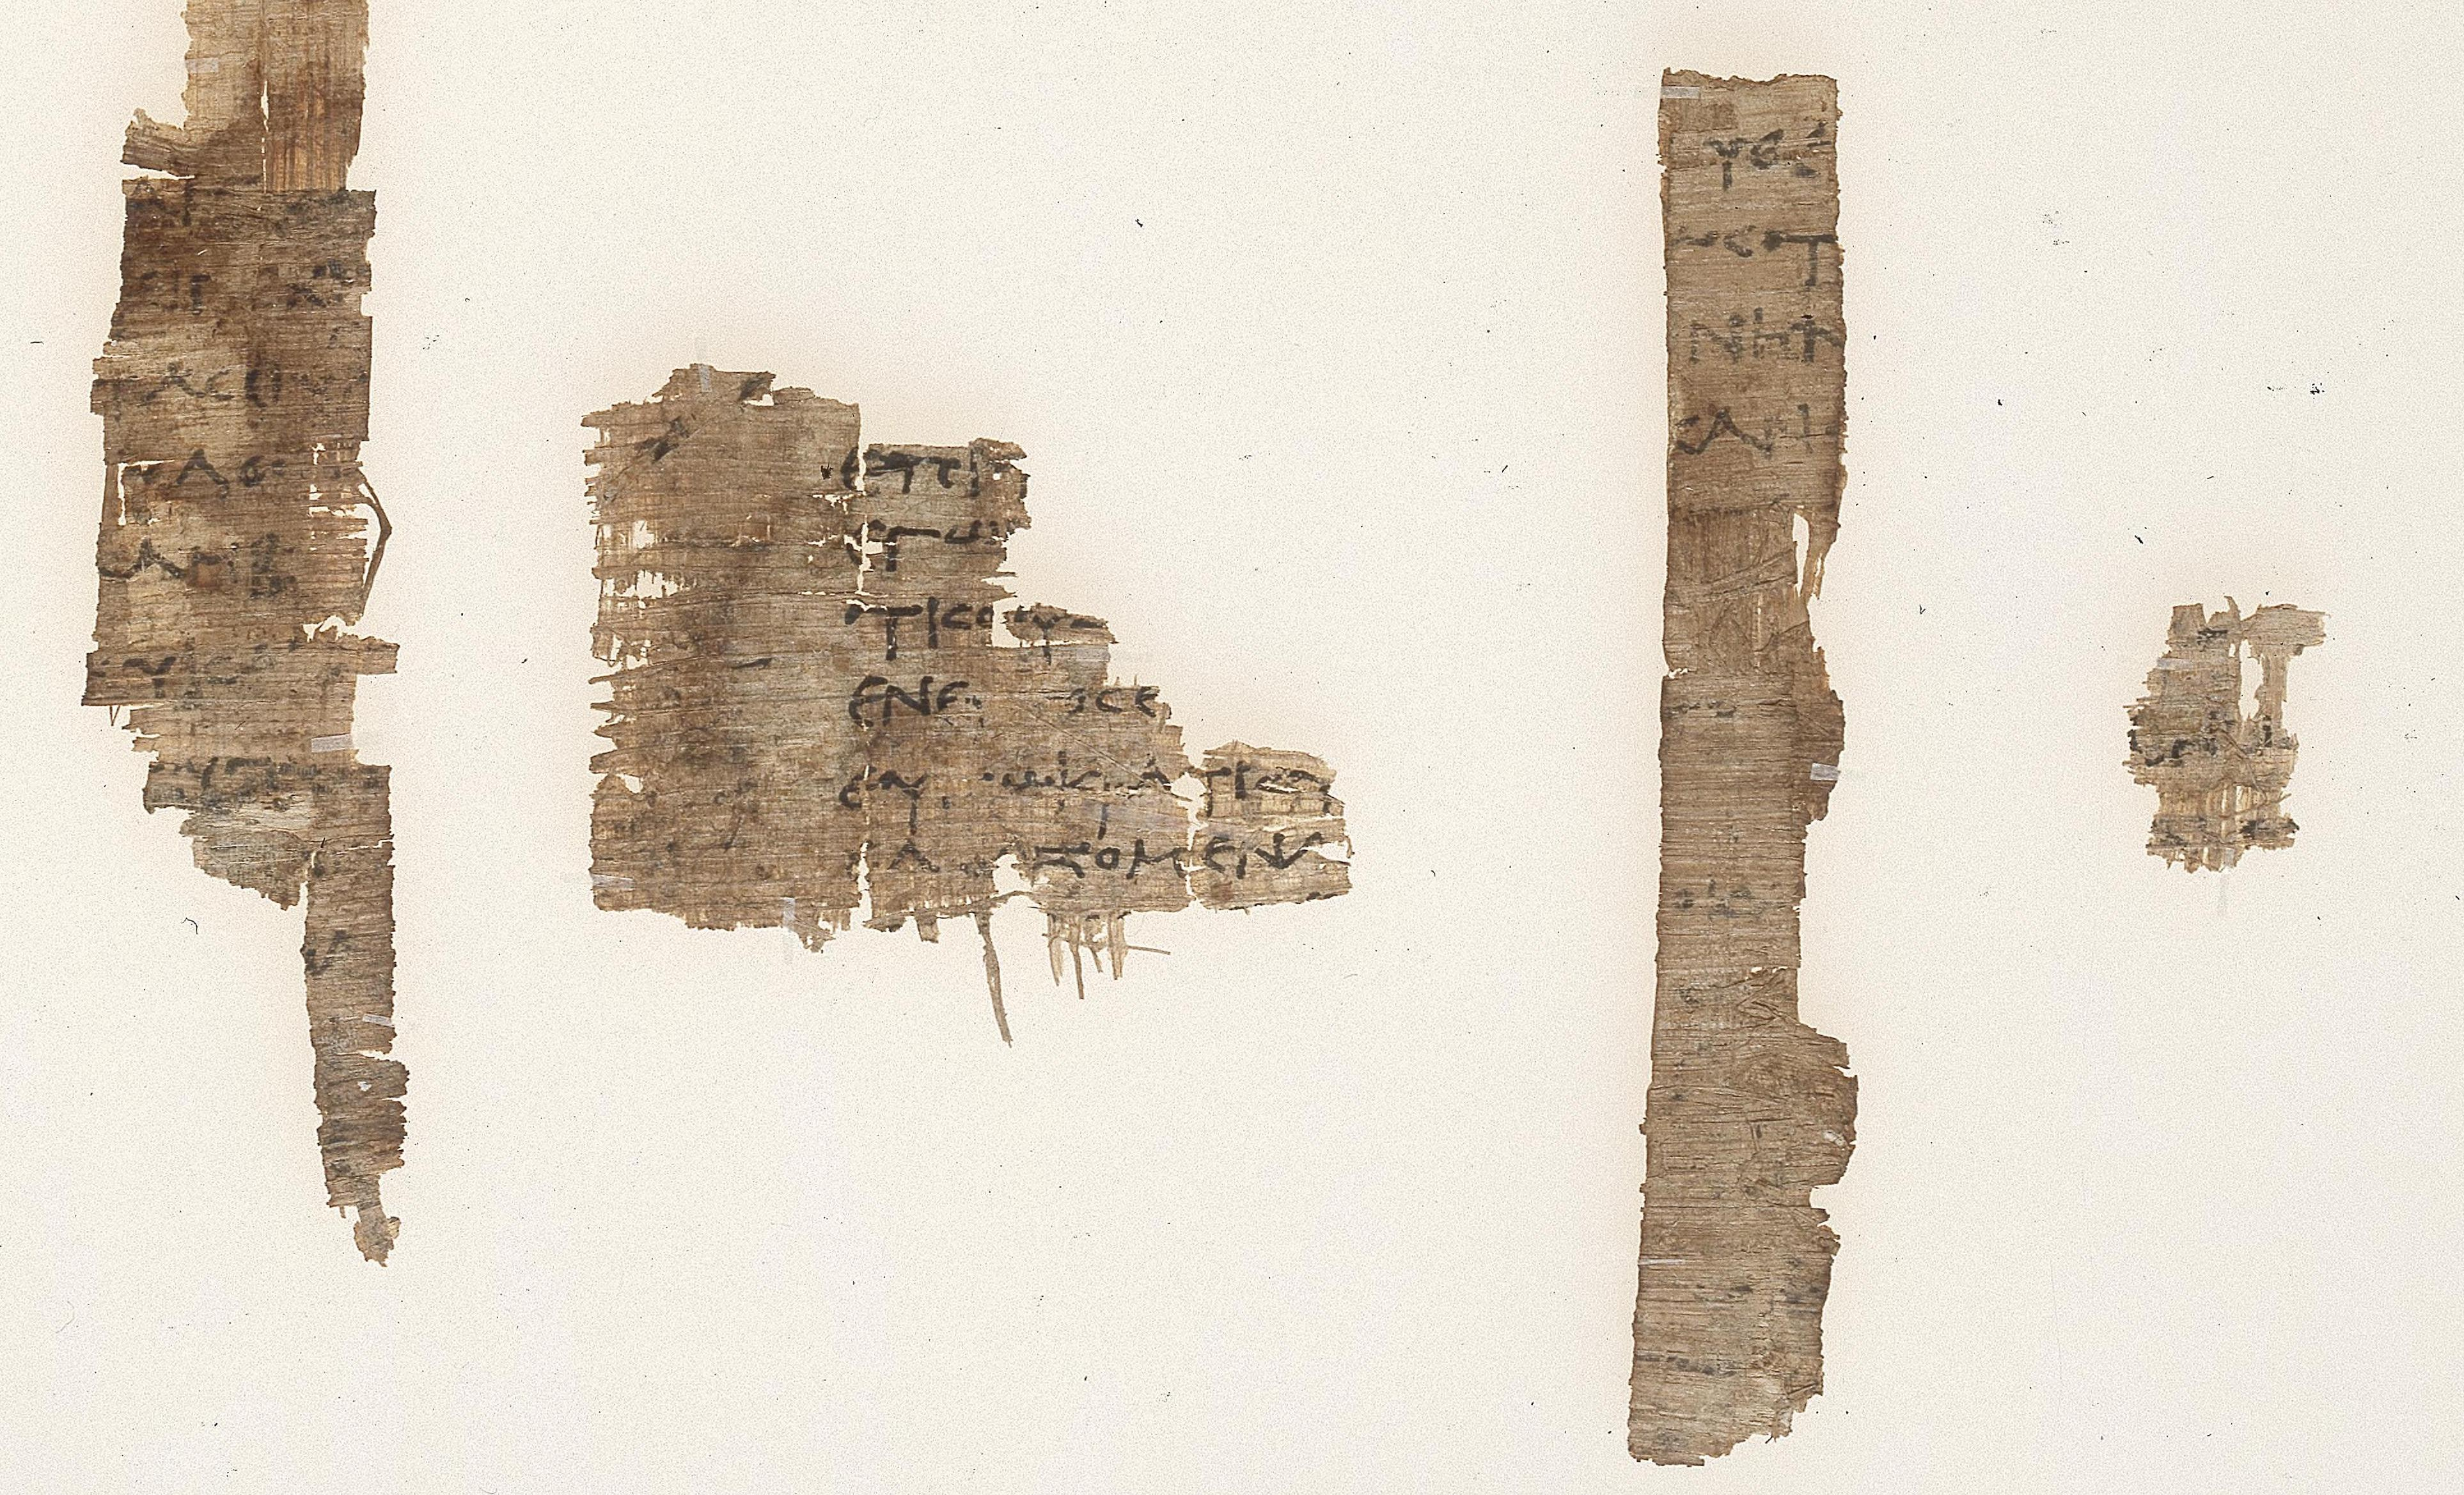
\includegraphics[width=\textwidth]{papyri_sample.jpg}
	\caption{A papyri torn into several fragments}
\end{figure}
Deep Learning algorithms are among the commonly discussed types of algorithms when it comes to supporting papyrologists. Research has shown that the use of Deep Learning can increase the efficiency of papyrologists. However, even though the results are promising, there are still many unanswered questions that we do not understand. Once a better understanding of the features is obtained, the algorithms can increase the papyrologist's efficiency by a greater chance. 


\section{Contribution}
The general objective of this thesis is to make the work of papyrologists easier and increase their efficiency
by partially automating the reassembling process. To this end, an algorithm is designed to infer a
smaller sub-selection of fragments with a high likelihood of being a potential fit. In the following, this
algorithm is called puzzle-helper. Additionally, the thesis explores the use of papyrus fibers to determine an accurate spatial position of two potential matching fragments. Also, using deep learning implies that a vast amount of (labeled) data is required. The database from the University of Michigan offers plenty of it. Once the data is downloaded, it must be correctly preprocessed, like removing low contrast images or labeling the data. In particular, this thesis is centered around the following research questions:
\begin{questions}
	\item  Does the puzzle-helpers-accuracy differ significantly when only the text or only the fibers are used as input as opposed to the unprocessed data?	
	\item  With the help of papyrus fibers, is it possible to determine the position of a fragment out of several matching candidates?	
\end{questions}


\section{Outline}
In the Chapter \ref{chap:intro}, the context of this master thesis was explained, and the research questions got defined. In the following, it is explained how the thesis is structured. Chapter \ref{chap:stateArt} presents groundbreaking work in all areas that are relevant for this thesis. That includes binarization, inpainting, and deep metric learning. The chapter's goal is to show the reader a quick overview of actual results in the field of historical fragment retrieval. Chapter \ref{chap:puzzleHelper} aims to explain how a ground truth is computed with the help of Deep Metric Learning (DML) for comparison later results. In Chapter \ref{chap:separating} the reader will learn how different datasets are obtained with the help of binarization and inpainting techniques. Furthermore, it is stated how results differ if the DML algorithm of the previous chapter is evaluated onto the different datasets. The results of the best-performing dataset from the previous chapter are used to determine spatial positions of potential matching candidates. That approach is explained in the Chapter \ref{chap:fibers}. A discussion about how the results of the different chapters determine the other results is stated in Chapter \ref{chap:discussion}. Finally, a conclusion is presented in Chapter \ref{chap:conclusion}, where the reader will be informed about lessons learned and potential future work.